\chapter{Methodology and Process}

The goal of this chapter is to outline which formal methods were selected for the development of this project, including the development process model, tools used, planning and estimations, as well as the risks involved with the project and how the team dealt with said risks. Furthermore, the methodology for achieving the goal of measuring and comparing different solutions is outlined.

\section{Agile Iterative Process}

The Agile Iterative Process\cite{raj13} (AIP) was chosen early on in development due to it's simplicity and natural fit with the developers usual preferred workflow. Some aspects of AIP were omitted to reduce unnecessary work overhead, such as a full complex software change process, and a dedicated process manager.

\subsection{Iterations}

The length of each iteration of the work process varied over the course of development due to changes in available work time, however it was agreed to be set to two weeks once full time was allotted to development. A time span of two weeks was chosen due to a natural fit with bi-weekly supervisor meetings and updates, with the goal being to have a run-able demonstration available for each meeting. Prior to full time work, no set iteration time span was decided, due to the unpredictability of available time.

\subsection{Product Manager and Users}

As with many projects of this nature, that being a student project, the product manager and users have in practice been the developers themselves. This does come with some difficulties, in particular in the role as users, as the developers might have some bias when considering the system from an outside black-box perspective, which could impact how the systems behaviour is viewed.

\subsection{Backlog}

The project backlog was initially based on a GitHub project\cite{githubprojects} which was used to track each tasks in the backlog. Each developer wrote in a set of tasks which were to be completed, and was then assigned a number of them. However, due to the simplicity of the system and short time span of development, the developers found it easier to merely maintain mental notes of the backlog instead, though the actual backlog tasks in the GitHub project were closed as they were completed in order to provide some overview on how close the project was to completion.

\section{Project Estimations}

\subsection{Gantt Diagram}

A Gantt Diagram was created early in development in order to maintain a time table, such that it would be possible to track whether or not the project was behind, on, or ahead of schedule. The milestones of the first half of the diagram was based on supervisor lectures in related areas, while the second half was loosely estimated based on previous experience. Initially completed tasks were filled in, but this practice was abandoned during the later stages of development, as it was deemed unnecessary as the team could easily manage who had worked on what due to the small team size and frequent meetings.

\begin{figure}[ht]
    \centering
    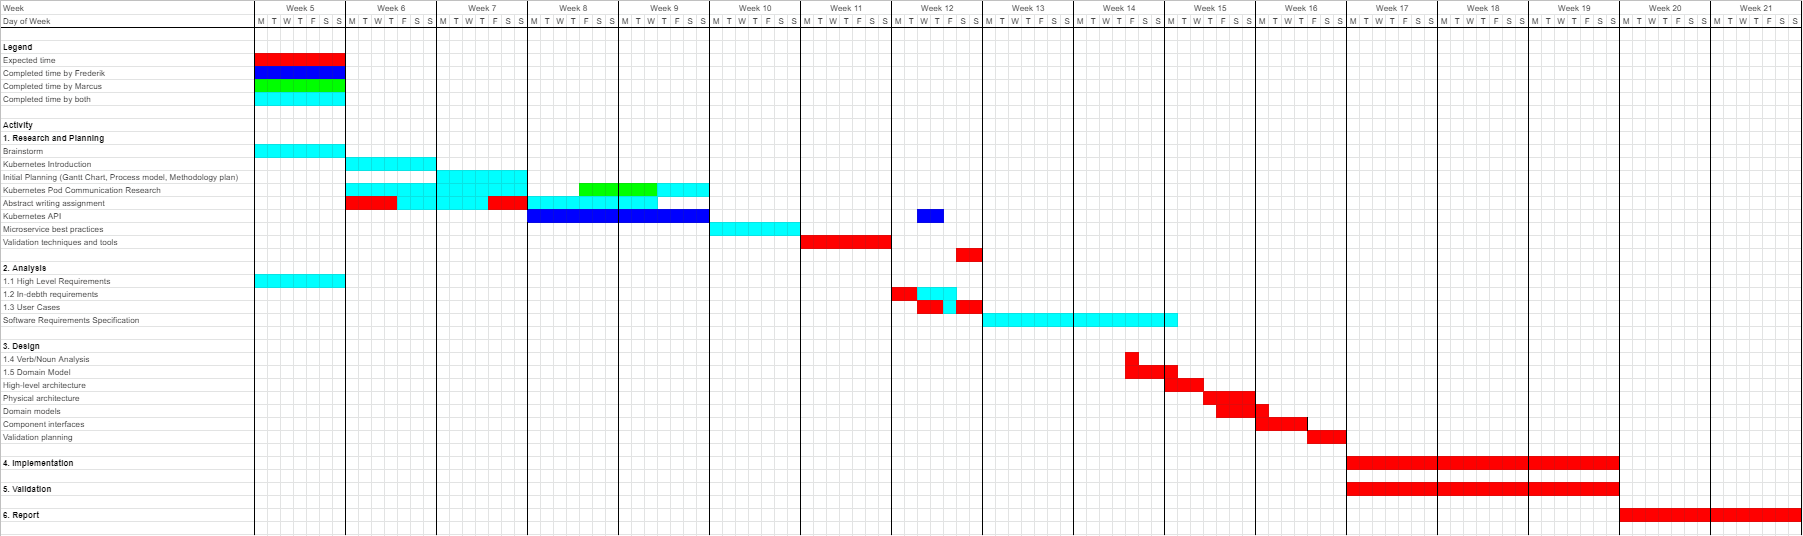
\includegraphics[width=\textwidth]{Pictures/Gantt.png}
    \caption{Gantt Diagram showing the general estimated time table between week 5 and week 21, with research and planning occuring between week 5 and week 11, analysis between 12 and 14, design in week 15 and 16, implementation and validation from from week 17 to 19, and finally report writing at the end in week 20 and 21. A larger more readable version is available as \ref{fig:ganttLarge}}
    \label{fig:gantt}
\end{figure}

\section{Risks}

Naturally any project carries risks. A few in particular were identified as the most threatening towards this project, mostly relating to the inherent unpredictability of software, unfamiliarity with the technologies involved, and the ever-endless Covid-19 quarantine taking a toll on the mental health of the developers.

\begin{table}[H]
\begin{tabularx}{\textwidth}{|l|X|m{3.25cm}|}
\hline
ID  & Description & Mitigation Strategy \\ \hline\hline
R01 & The product would not be completed in time due to poor time management. Software development is known to be volatile and difficult to estimate, and so it happens that projects fail to be finished in time. & Reduction through estimating a tentative time table.          \\ \hline
R02 & The project would fail to reach its goals due to technical difficulties with unfamiliar technologies. Neither developer are very experienced with the technologies involved beyond the basics, and there could easily unforeseen consequences with the choice of technology.                                         & Reduction through prototyping a rudimentary system.           \\ \hline
R03 & Lack of motivation due to mental health impact of quarantine would impact project quality. While both developers have dealt with the quarantine somewhat well prior to the project, the prolonged quarantine can easily affect motivation to get work done.                                                                                & Acceptance          \\ \hline
R04 & The project exam is failed. This would be a critical failure of the project as a whole, though it is unlikely to occur unless everything that could go wrong did go wrong.                                                                                                                                         & Avoidance through work.           \\ \hline
\end{tabularx}
\caption{Table of the four most major estimated project risks. Each risk has an ID, a description and a mitigation strategy.}
\label{tab:risks}
\end{table}

\newpage
Each risk is assessed on likelihood to occur and severity of consequence on a scale between 1 and 5 using a Risk Assessment Matrix. The colors represent the severity of the potential risk, taking likelihood and consequence into account. Green is low, yellow moderate, orange high , while red is extreme.

\begin{figure}[H]
    \centering
    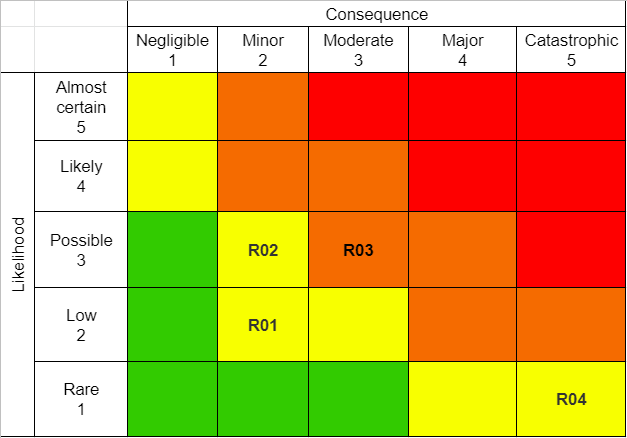
\includegraphics[scale=0.4]{Pictures/RiskAssesmentMatrix.png}
    \caption{The Risk Assessment Matrix for the project. It can be seen how no risks are within the red zone, but R01, R02, and R04 lies within the yellow zone. R03 lies within the orange zone, and is estimated to be the greatest risk to the project.}
    \label{fig:riskmatrix}
\end{figure}

\section{Conclusion}

The development methodologies and processes have overall been highly agile, with little in terms of significant specific plans for what should be done when, and how it should be done, aside from Gantt diagram which ended up mostly as a loose time table. A slightly toned down variant of the Agile Iterative Process was used for development, with a varying iteration time span until the later stages, where full time work was a possibility, and the time span was set to two weeks. The goal of each iteration was to end with a presentable demo for the bi-weekly supervisor meetings. A written backlog was initially used, but soon grew out of favor as the small team size had no real need for it. There were some risks with the project, including unpredictable development times, difficulties with technology, and outright failing the final exam. These were, however, only estimated to be of only minor concern, while the ongoing Covid-19 quarantine and its impact on mental health was estimated to be a much more significant threat, in particular as there is not much which can be done to prevent it.